\documentclass[11pt,letterpaper]{article}

\newenvironment{proof}{\noindent{\bf Proof:}}{\qed\bigskip}

\newtheorem{theorem}{Theorem}
\newtheorem{corollary}{Corollary}
\newtheorem{lemma}{Lemma} 
\newtheorem{claim}{Claim}
\newtheorem{fact}{Fact}
\newtheorem{definition}{Definition}
\newtheorem{assumption}{Assumption}
\newtheorem{observation}{Observation}
\newtheorem{example}{Example}
\newcommand{\qed}{\rule{7pt}{7pt}}

\newcommand{\solution}[4]{
\thispagestyle{plain} 
\newpage
\setcounter{page}{1}
\noindent
\begin{center}
\framebox{ \vbox{
\vspace{4mm}
\vspace{0.2in} 
{\centering \large\mbox{#3}}\\
\vspace{0.1in}
{#1 \hfill {Date: #2}}
}}
\end{center}
\markright{#1}
}

\newenvironment{algorithm}
{\begin{center}
\begin{tabular}{|l|}
\hline
\begin{minipage}{1in}
\begin{tabbing}
\quad\=\qquad\=\qquad\=\qquad\=\qquad\=\qquad\=\qquad\=\kill}
{\end{tabbing}
\end{minipage} \\
\hline
\end{tabular}
\end{center}}

\def\Comment#1{\textsf{\textsl{$\langle\!\langle$#1\/$\rangle\!\rangle$}}}



\usepackage{graphicx, amssymb, amsmath, listings, float, mathtools}
\usepackage{color, url}
\lstset{language = Python}
\lstset{breaklines}
\lstset{extendedchars=false}
\usepackage{xcolor}

\oddsidemargin 0in
\evensidemargin 0in
\textwidth 6.5in
\topmargin -0.6in
\textheight 9.0in

\newsavebox\MBox
\newcommand\Cline[2][red]{{\sbox\MBox{$#2$}%
  \rlap{\usebox\MBox}\color{#1}\rule[-2\dp\MBox]{\wd\MBox}{2pt}}}

\begin{document}

\solution{\large Jifu Zhao}{\large 10/30/2016}{\bf \Large ECE 544NA \hspace{0.5cm} 
		Fall 2016 \hspace{0.5cm} Assignment 4}

\section*{\Large I. Pencil-and-Paper}
Suppose $(V, H)$ denote the visible and hidden random variable which takes values ($v \in \{0, 1\}^m$, $h \in \{0, 1\}^n$). And the joint probability is $p(v, h; \theta) = \frac{1}{Z}e^{-E(v, h; \theta)}$, where E is the energy function:
\begin{equation}
\begin{split}
E(v, h; \theta) & = -\sum_{i=1}^n \sum_{j=1}^m w_{ij} h_i v_j - \sum_{j=1}^m b_j v_j - \sum_{i=1}^n c_i h_i \\
				& = -(\mathbf{v^T W h + v^T b + h^T c})
\end{split}
\end{equation}
where $Z = \sum_v \sum_h e^{-E(v, h, \theta)}$ and $\theta = (W, b, c)$.


\begin{description}
%%%%%%%%%%%%%%%%%%%%%%%%%%%%%%%%%%%%%%%%%%%%%%%%%%%%%%%%%%%%%%%%%%%%%%%%%%%%%%%%%%%%%%%%%
% Problem 1
\item{\bf \large 1. } Find $p(v|h, \theta)$ and $\mathbb{E}(v|h, \theta)$.

From the structure of RBM, it means that the hidden variables are independent given the state of the visible variables and the visible variables are independent given the state of the hidden variables. In this way,
\begin{equation}
\begin{split}
\Cline[red]{p(v| h, \theta)} 
	& = \frac{p(v, h | \theta)}{p(h| \theta)} \\
	& = \frac{\prod_i^n \prod_j^m p(v_j, h_i|\theta)}{\sum_{v} \prod_i^n \prod_j^m p(v_j, h_i|\theta)}
\end{split}
\end{equation}

So, we also have:
\begin{equation}
\mathbb{E}(v|h, \theta) =  sigmoid(W^T h + b)
\end{equation}
(The prof will be shown later)

For $p(v_j|h)$, 
\begin{equation}
p(v_j|h) = \frac{p(v_j, h)}{p(h)} = \frac{p(v_j, h)}{p(v_j=0, h) + p(v_j=1, h)}
\end{equation}

Since that $p(v_j=0, h) = \frac{1}{Z}e^{-E(v_j=0, h; \theta)}$ and $p(v_j=1, h) = \frac{1}{Z}e^{-E(v_j=1, h; \theta)}$. From equation (1), we can think $E(v, h; \theta) = v_j \alpha_j + \beta$, where $\beta$ doesn't contain $v_j$. 

In this way, we have:
\begin{equation}
\begin{split}
p(v_j|h) & = \frac{p(v_j, h)}{p(v_j=0, h) + p(v_j=1, h)} \\
		 & = \frac{exp(-v_j \alpha_j - \beta)}{exp(-\beta) + exp(-\alpha_j - \beta)} \\
		 & = \frac{exp(-v_j \alpha_j)}{1 + exp(-\alpha_j)}
\end{split} 
\end{equation}

So, we have
\begin{equation}
p(v_j = 1|h) = \frac{exp(-\alpha_j)}{1 + exp(-\alpha_j)} = \frac{1}{1 + exp(\alpha_j)}
\end{equation}
and 
\begin{equation}
p(v_j = 0|h) = \frac{1}{1 + exp(-\alpha_j)} = 1 - \frac{1}{1 + exp(\alpha_j)}
\end{equation}

From equation (1), we can see that $\alpha_j = -\sum_{i=1}^n w_{ij}h_i - b_j$, so we can see that:
\begin{equation}
\Cline[red]{p(v_j = 1|h) = sigmoid(-\alpha_j) = sigmoid(\sum_{i=1}^n w_{ij}h_i + b_j)}
\end{equation}
and 
\begin{equation}
\Cline[red]{p(v_j = 0|h) = 1 - sigmoid(-\alpha_j) = 1 - sigmoid(\sum_{i=1}^n w_{ij}h_i + b_j)}
\end{equation}

From equation (8) and (9), we can see that:
\begin{equation}
\mathbb{E}(v_j|h, \theta) = 1 \cdot p(v_j = 1|h, \theta) + 0 \cdot p(v_j = 0|h, \theta) = sigmoid(\sum_{i=1}^n w_{ij}h_i + b_j)
\end{equation}
In the vector format:
\begin{equation}
\Cline[red]{\mathbb{E}(v|h, \theta) = sigmoid(W^T h + b)}
\end{equation}\\

%%%%%%%%%%%%%%%%%%%%%%%%%%%%%%%%%%%%%%%%%%%%%%%%%%%%%%%%%%%%%%%%%%%%%%%%%%%%%%%%%%%%%%%%%
% Problem 2
\item{\bf \large 2. } Find $p(h|v, \theta)$ and $\mathbb{E}(h|v, \theta)$.

Similar to the procedures in 1, since that the hidden variables are independent given the state of the visible variables. In this way,
\begin{equation}
\begin{split}
\Cline[red]{p(h| v, \theta)} 
	& = \frac{p(v, h | \theta)}{p(v| \theta)} \\
	& = \frac{\prod_i^n \prod_j^m p(v_j, h_i|\theta)}{\sum_{h} \prod_i^n \prod_j^m p(v_j, h_i|\theta)}
\end{split}
\end{equation}

So, we also have:
\begin{equation}
\mathbb{E}(h|v, \theta) =  sigmoid(W v + c)
\end{equation}

For $p(h_i|v)$, 
\begin{equation}
p(h_i|v) = \frac{p(h_i, v)}{p(v)} = \frac{p(h_i, v)}{p(h_i=0, v) + p(h_i=1, v)}
\end{equation}

Since that $p(h_i=0, v) = \frac{1}{Z}e^{-E(v, h_i=0; \theta)}$ and $p(h_i=1, v) = \frac{1}{Z}e^{-E(v, h_i=1; \theta)}$.
From equation (1), we can think $E(v, h; \theta) = h_i \gamma_i + \beta'$, where $\beta'$ doesn't contain $h_i$. In this way, we have:
\begin{equation}
\begin{split}
p(h_i|v) & = \frac{p(h_i, v)}{p(h_i=0, v) + p(h_i=1, v)} \\
		 & = \frac{exp(-h_i \gamma_i - \beta')}{exp(-\beta') + exp(-\gamma_i - \beta')} \\
		 & = \frac{exp(-h_i \gamma_i)}{1 + exp(-\gamma_i)}
\end{split} 
\end{equation}

So, we have
\begin{equation}
p(h_i=1|v) = \frac{exp(-\gamma_i)}{1 + exp(-\gamma_i)} = \frac{1}{1 + exp(\gamma_i)}
\end{equation}
and 
\begin{equation}
p(h_i=0|v) = \frac{1}{1 + exp(-\gamma_i)} = 1 - \frac{1}{1 + exp(\gamma_i)}
\end{equation}

From equation (1), we can see that $\gamma_i = -\sum_{j=1}^m w_{ij}v_j - c_i$, so we can see that:
\begin{equation}
\Cline[red]{p(h_i=1|v) = sigmoid(-\gamma_i) = sigmoid(\sum_{j=1}^m w_{ij}v_j + c_i)}
\end{equation}
and 
\begin{equation}
\Cline[red]{p(h_i=0|v) = 1 - sigmoid(-\gamma_i) = 1 - sigmoid(\sum_{j=1}^m w_{ij}v_j + c_i)}
\end{equation}

From equation (18) and (19), we can see that:
\begin{equation}
\mathbb{E}(h_i|v, \theta) = 1 \cdot p(h_i=1|v, \theta) + 0 \cdot p(h_i=0|v, \theta) = sigmoid(\sum_{j=1}^m w_{ij}v_j + c_i)
\end{equation}
In the vector format:
\begin{equation}
\Cline[red]{\mathbb{E}(h|v, \theta) = sigmoid(W v + c)}
\end{equation}\\

%%%%%%%%%%%%%%%%%%%%%%%%%%%%%%%%%%%%%%%%%%%%%%%%%%%%%%%%%%%%%%%%%%%%%%%%%%%%%%%%%%%%%%%%%
% Problem 3
\item{\bf \large 3. } Compute $\frac{\partial \mathcal{L}(D|\theta)}{\partial W_{ij}}$, $\frac{\partial \mathcal{L}(D|\theta)}{\partial b_{j}}$ and $\frac{\partial \mathcal{L}(D|\theta)}{\partial c_{i}}$

Now, suppose the given dataset is $D=\{v_1, v_2, \cdots, v_N\}$, then the log-likelihood can be calculated as:
\begin{equation}
\mathcal{L}(D|\theta) = \sum_{t=1}^N log(p(v_t|\theta))
\end{equation}

Since that 
\begin{equation}
p(v_t|\theta) = \sum_{h_t} p(v_t, h_t|\theta) = \frac{1}{Z}\sum_{h_t} exp(-E(v_t, h_t; \theta))
\end{equation}
where $Z = \sum_{v_t}\sum_{h_t}exp(-E(v_t, h_t; \theta))$

we can get:
\begin{equation}
\begin{split}
log(p(v_t|\theta)) & = log(\frac{1}{Z}\sum_{h_t} exp(-E(v_t, h_t; \theta))) \\
				   & = log(\sum_{h_t}exp(-E(v_t, h_t; \theta))) - log(\sum_{v_t}\sum_{h_t}exp(-E(v_t, h_t; \theta))) 
\end{split}
\end{equation}

So, to calculate the derivation, we can get:
\begin{equation}
\begin{split}
\frac{\partial log(p(v_t|\theta))}{\partial \theta} 
	& = \frac{\partial}{\partial \theta} log(\sum_{h_t}exp(-E(v_t, h_t; \theta))) - \frac{\partial}{\partial \theta} log(\sum_{v_t}\sum_{h_t}exp(-E(v_t, h_t; \theta)))  \\
	& = -\frac{1}{\sum_{h_t} e^{-E}} \sum_{h_t} e^{-E} \cdot \frac{\partial E}{\partial \theta} + 
		 \frac{1}{\sum_{v_t}\sum_{h_t} e^{-E}} \sum_{v_t}\sum_{h_t} e^{-E} \cdot \frac{\partial E}{\partial \theta} \\
	& = -\frac{\sum_{h_t} e^{-E} \cdot \frac{\partial E}{\partial \theta}}{Z \cdot p(v_t|\theta)}
	    + \sum_{v_t}\sum_{h_t} \frac{e^{-E}}{Z} \cdot \frac{\partial E}{\partial \theta} \\
	& = -\sum_{h_t} p(h_t|v_t, \theta) \cdot \frac{\partial E}{\partial \theta}
	    +\sum_{v_t}\sum_{h_t} p(v_t, h_t|\theta) \cdot \frac{\partial E}{\partial \theta} \\
	& = \Cline[red]{-\sum_{h} p(h|v) \cdot \frac{\partial E(v, h)}{\partial \theta}
	    +\sum_{v}\sum_{h} p(v, h) \cdot \frac{\partial E(v, h)}{\partial \theta}}
\end{split}
\end{equation}

From equation (25), we can get:
\begin{equation}
\begin{split}
\frac{\partial \mathcal{L}(D|\theta)}{\partial W_{ij}} 
	& = -\sum_{h} p(h|v) \cdot \frac{\partial E(v, h)}{\partial w_{ij}}
	    +\sum_{v}\sum_{h} p(v, h) \cdot \frac{\partial E(v, h)}{\partial w_{ij}} \\
	& = \sum_{h} h_i v_j \cdot p(h|v) - \sum_h \sum_v h_i v_j \cdot p(v, h) \\
	& = \Cline[red]{p(h_i=1|v) \cdot v_j - \sum_v p(v) \cdot p(h_i=1|v) \cdot v_j} \\
	& = \Cline[red]{p(h_i=1|v) \cdot v_j - \mathbf{E}[v_j h_i]} 
\end{split}
\end{equation}

In the similar way, we can have:
\begin{equation}
\begin{split}
\frac{\partial \mathcal{L}(D|\theta)}{\partial b_{j}} 
	& = \sum_{h} v_j \cdot p(h|v) - \sum_h \sum_v v_j \cdot p(v, h) \\
	& = \Cline[red]{v_j - \sum_v p(v) \cdot v_j} \\
	& = \Cline[red]{v_j - \mathbf{E}[v_j]}
\end{split}
\end{equation}

\begin{equation}
\begin{split}
\frac{\partial \mathcal{L}(D|\theta)}{\partial c_{i}} 
	& = \sum_{h} h_i \cdot p(h|v) - \sum_h \sum_v h_i \cdot p(v, h) \\
	& = \Cline[red]{p(h_i=1|v) - \sum_v p(v) \cdot p(h_i=1|v)} \\
	& = \Cline[red]{p(h_i=1|v) - \mathbf{E}[h_i]}
\end{split}
\end{equation}

%%%%%%%%%%%%%%%%%%%%%%%%%%%%%%%%%%%%%%%%%%%%%%%%%%%%%%%%%%%%%%%%%%%%%%%%%%%%%%%%%%%%%%%%%
% Problem 4
\item{\bf \large 4. } Contrastive divergence

From equation (26), (27) and (28), we can find that $p(v, h)$ is actually a computationally intractable term. To solve this problem, we should consider 1-step contrastive divergence to solve this problem.

Considering Hinton approximation:
\begin{equation}
\mathbf{E}[v_j h_i] \simeq \mathbf{E}[v_j|h] \mathbf{E}[h_i|v]
\end{equation}

And the k-step contrastive divergence is:
\begin{equation}
CD_k(\theta, v^{(0)}) = -\sum_h p(h|v^{(0)})\frac{\partial E(^{(0)}, h)}{\partial \theta}
					+\sum_h p(h|v^{(k)})\frac{\partial E(v^{(k)}, h)}{\partial \theta}
\end{equation}


First, choose one visible data $v^{(0)}$ from the given training set, sample hidden nodes $h^{(0)}$ according to $p(h|v^{(0)})$. Then, calculate the probability $p(v|h^{(0)})$ using the sampled hidden nodes, and then reconstruct the visible nodes $v^{(1)}$ according to $p(v|h^{(0)})$. Finally, calculate the probability of $p(h^{(1)}|v^{(1)})$. Using these result to approximate and calculate the update rules for $W$, $b$ and $c$.

{\bf Note:} The above method is for 1-step CD sampling, if needed, this procedure can be repeated k times.

\end{description}

\newpage
\section*{\Large II. Code-from-Scratch}

\subsection*{\large 1. Methods}

The algorithm for RBM is relatively simple: First initialize all the parameters including $W$, $b$ and $c$. Then given any visible sample $v_0$,  first sample $h_0$ according to $p(h_0|v_0)$. Then, reconstruct $v_1$ according to $p(v_1|h_0)$. Finally, re-sample $h_1$ according to $p(h_1|v_1)$. Finally, update all the parameters including $W$, $b$ and $c$. Repeat this procedure enough times, then you can get the desired result. The detailed structure of the code is shown in Figure \ref{fig:structure}. 

In the class RBM(), there are several functions such as train(), \_initialize(), update\_h(), update\_v(), gradient() and sigmoid(). Function \_initialize() is used to initialize all parameters. Then function train() is used to train the RBM model, it will call the functions update\_h(), update\_v(), gradient() and sigmoid() to update all parameters. In this code, RBM can be trained through single input data, or through mini-batch learning.

\begin{figure}[H]
\centering
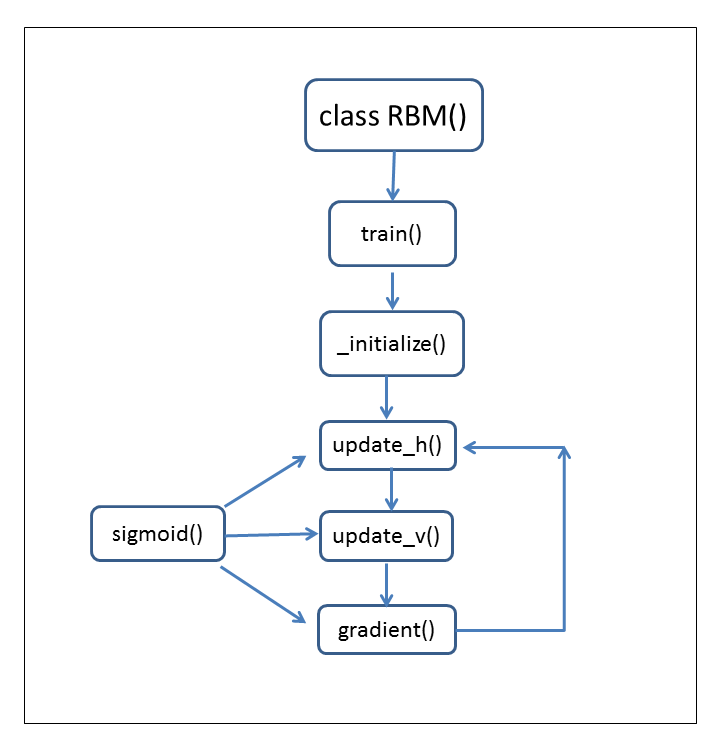
\includegraphics[width=0.8\textwidth]{./figures/ECE544hw4.png}\
\caption{\label{fig:structure} Overall Structure for RBM}
\end{figure}

\subsection*{\large 2. Results}

\noindent {\bf Note: } In the following result section, due to different initialization, the final result may be different for each running.

In this part, using the code illustrated in Figure \ref{fig:structure} and updating RBM model using single input image, the first 64 of the 200 learned filters are shown in Figure \ref{fig:single_filter}.

\begin{figure}[H]
\centering
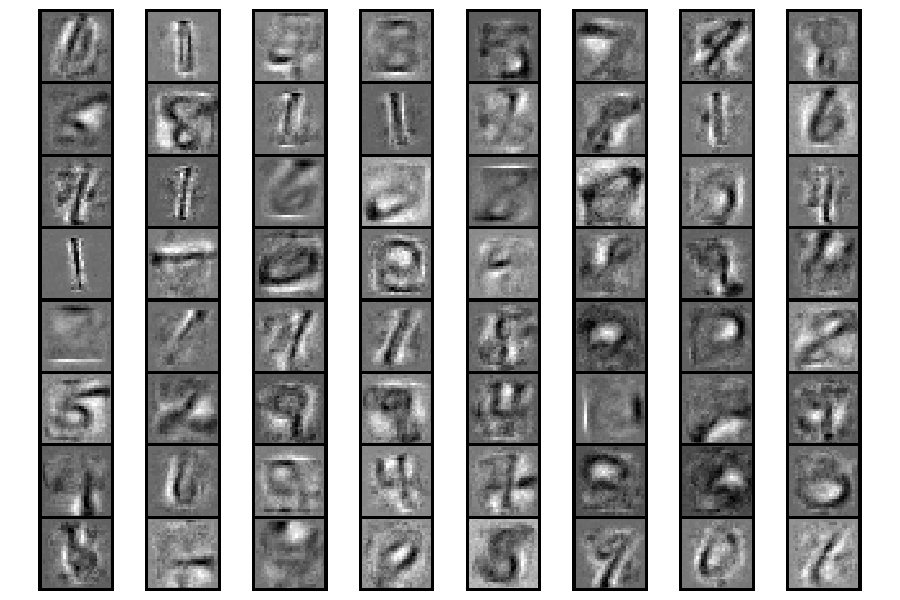
\includegraphics[width=1.0\textwidth]{./figures/filter.pdf}\
\caption{\label{fig:single_filter} Learned Filter}
\end{figure}

In Figure \ref{fig:single_filter}, all the learned filters shown some interesting phenomenon, most of them shown some clear digits. 

As a comparison, we also tried using 10-mini-batch learning method, the first 64 learned filters are shown in Figure \ref{fig:batch_filter}. As you can see, using mini-batch, the learned filter is not as clear as shown in Figure \ref{fig:single_filter}.

\begin{figure}[H]
\centering
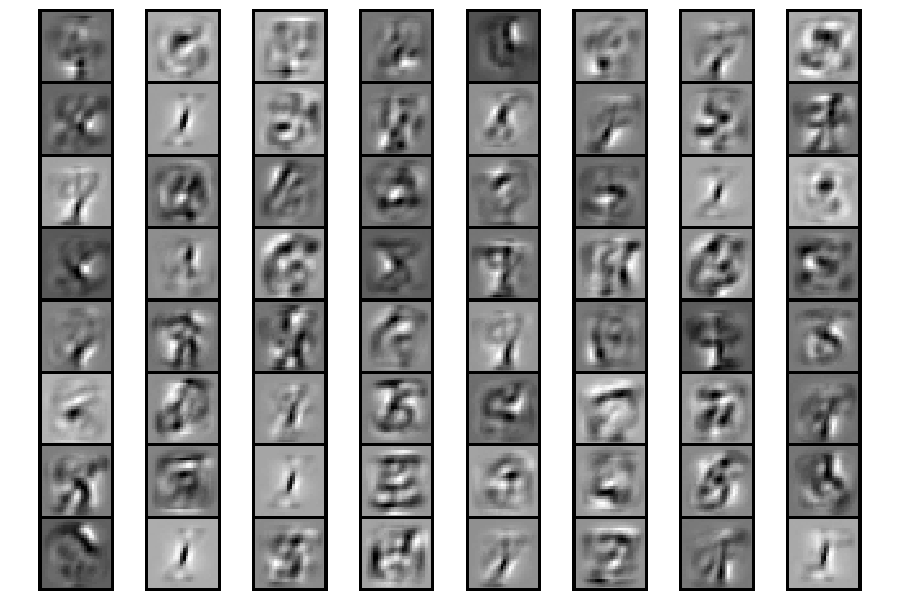
\includegraphics[width=1.0\textwidth]{./figures/filter_batch.pdf}\
\caption{\label{fig:batch_filter} Learned Filter}
\end{figure}

\newpage
\section*{\Large III. TensorFlow}

\subsection*{\large 1. Methods}

(1) In this part, the RBM model is re-written in TensorFlow. The overall structure is very similar. However, considering the characteristic of TensorFlow, there aren't so many functions as shown in Figure \ref{fig:structure}. Instead, the overall structure is shown in Figure \ref{fig:tf_structure}.

\begin{figure}[H]
\centering
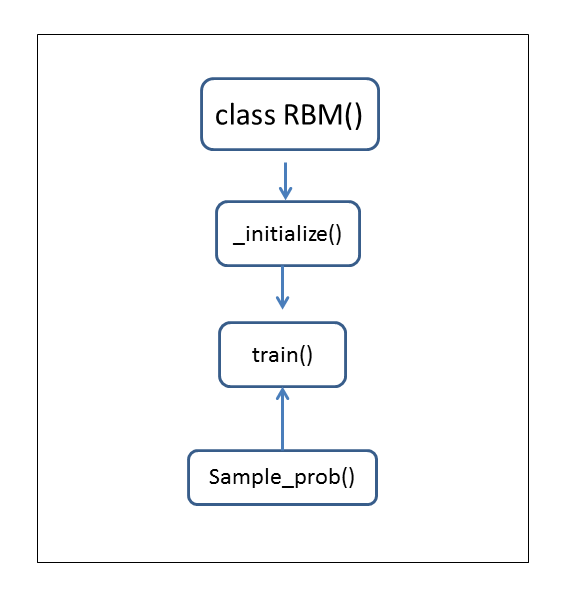
\includegraphics[width=0.8\textwidth]{./figures/ECE544hw4(2).png}
\caption{\label{fig:tf_structure} Overall Structure for TensorFlow RBM}
\end{figure}

In RBM part, we use function \_initialize() to initialize all parameters and create Variables and placeholders. Then, using function train() to train the model. In this process, function sample\_prob() is used to sample the Bernoulli distribution. 

More specifically, tf.nn.sigmoid() is used to compute sigmoid probability, tf.truncated\_normal() is used to initialize parameters and assign\_add() is used to update parameters. In addition, tf.nn.relu() and tf.random\_uniform() is used to create function sample\_prob(). \\

\noindent (2) For the 10-way multi-class logistic regression part, we build a fully-connected neural network. The input can have 784 or 200 nodes, the output out has 10 nodes using a softmax() function. More specifically, in the part, we use tflearn.input\_data(), tflearn.fully\_connected(), tflearn.regression() and tflearn.DNN() to train the model. \\

\noindent (3) For the stacked RBM, in the first RBM, there is 784 visible nodes and 500 hidden nodes, so the total number of weights is:
\begin{equation}
784 \times 500 + 784 + 500 = 393284
\end{equation}

In the second RBM, there are 500 visible nodes and 200 hidden nodes, the total number of weights is:
\begin{equation}
500 \times 200 + 500 + 200 = 100700
\end{equation}

So the total weights for the whole stacked RBM is:
\begin{equation}
393284 + 100700 = 493984
\end{equation}\

\noindent {\bf Note: } in the above calculation, the bias term b and c for each RBM are also thought to be part of the weights.\\


\subsection*{\large 2. Results}

(1) In this part, using the raw image, image processed by single RBM, image processed by PCA and image processed by stacked RBM, we train a 1 layer neural network and calculate the training accuracy and testing accuracy. The result is shown in Table \ref{table:BESTacc}. 

\begin{table}[H]
	\centering
	\caption{Training and testing accuracy for different models}
	\label{table:BESTacc}	
	\begin{tabular}{c | c | c}
		\hline \hline
		Methods  	&	Training Accuracy 	&	Testing Accuracy \\[0.1cm]
		\hline
		Raw Image	&	92.99\%				& 	92.59\%			 \\[0.1cm]
		RBM			&	94.99\%				& 	94.93\%			 \\[0.1cm]
		PCA			& 	92.32\%				& 	92.07\%			 \\[0.1cm]
		Stacked RBM & 	96.35\%				& 	96.24\%			 \\[0.1cm]
		\hline	
	\end{tabular}
\end{table}

From Table \ref{table:BESTacc}, we can see that, the result from PCA is similar to the result from raw image. But using RBM and stacked RBM, the training accuracy and testing accuracy both get improved.\\

\noindent (2) Training and testing classification confusion matrix. (See next page)
\newpage
(a). For the raw image, the training and testing classification confusion matrix are shown in Figure \ref{fig:train_raw} and Figure \ref{fig:test_raw}.

\begin{figure}[H]
\centering
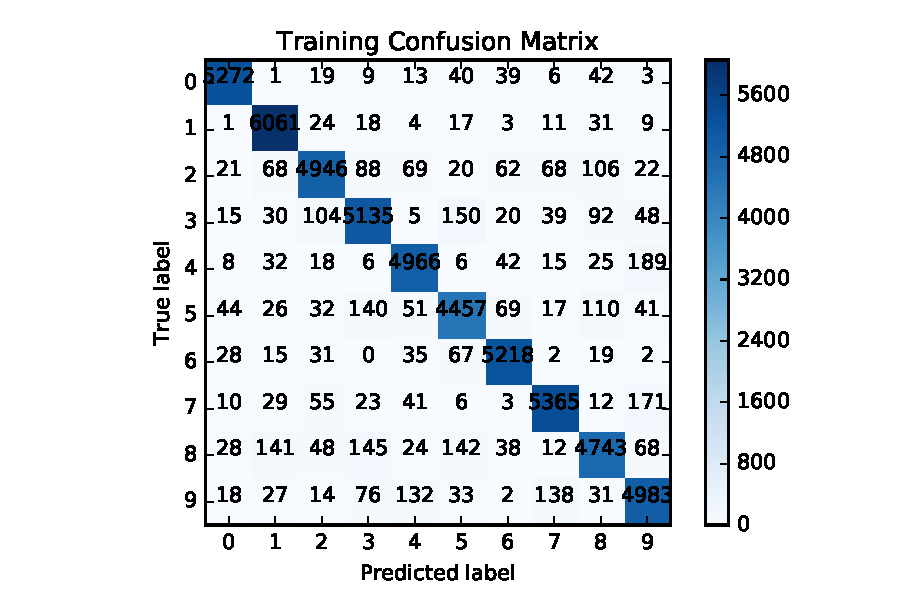
\includegraphics[width=0.85\textwidth]{./figures/train_raw.pdf}\
\caption{\label{fig:train_raw} Training Set Confusion Matrix Using Raw Image}
\end{figure}

\begin{figure}[H]
\centering
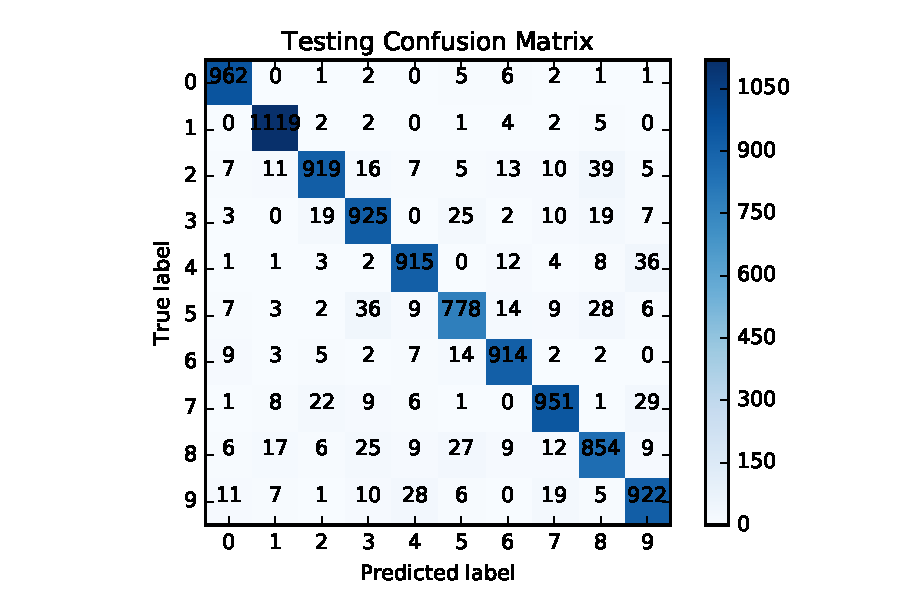
\includegraphics[width=0.85\textwidth]{./figures/test_raw.pdf}\
\caption{\label{fig:test_raw} Test Set Confusion Matrix Using Raw Image}
\end{figure}

(b). For the image processed by RBM, the training and testing classification confusion matrix are shown in Figure \ref{fig:train_rbm} and Figure \ref{fig:test_rbm}.

\begin{figure}[H]
\centering
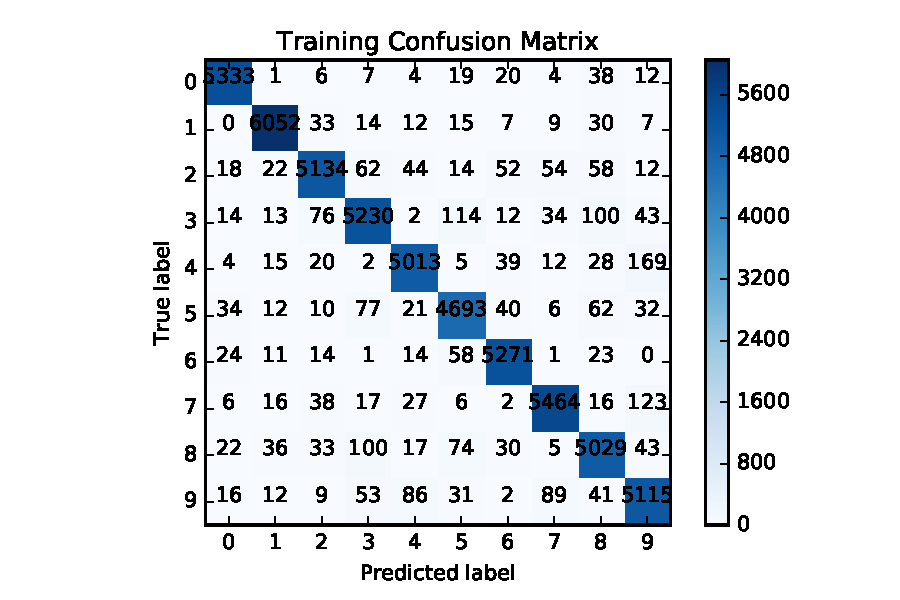
\includegraphics[width=0.85\textwidth]{./figures/train_rbm.pdf}\
\caption{\label{fig:train_rbm} Training Set Confusion Matrix Using RBM}
\end{figure}

\begin{figure}[H]
\centering
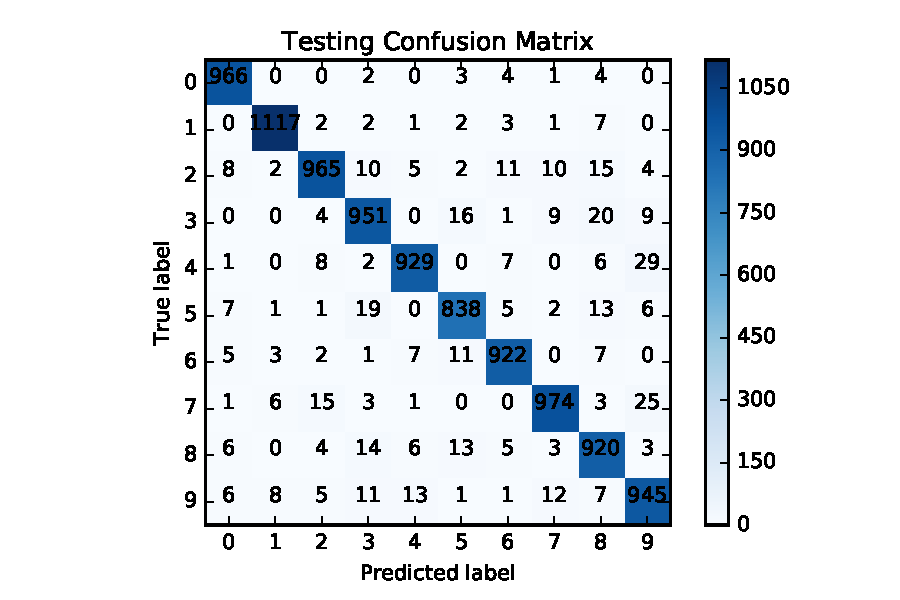
\includegraphics[width=0.85\textwidth]{./figures/test_rbm.pdf}\
\caption{\label{fig:test_rbm} Test Set Confusion Matrix Using RBM}
\end{figure}

(c). For the image processed by PCA, the training and testing classification confusion matrix are shown in Figure \ref{fig:train_pca} and Figure \ref{fig:test_pca}. (The PCA part is implemented using scikit-learn PCA)

\begin{figure}[H]
\centering
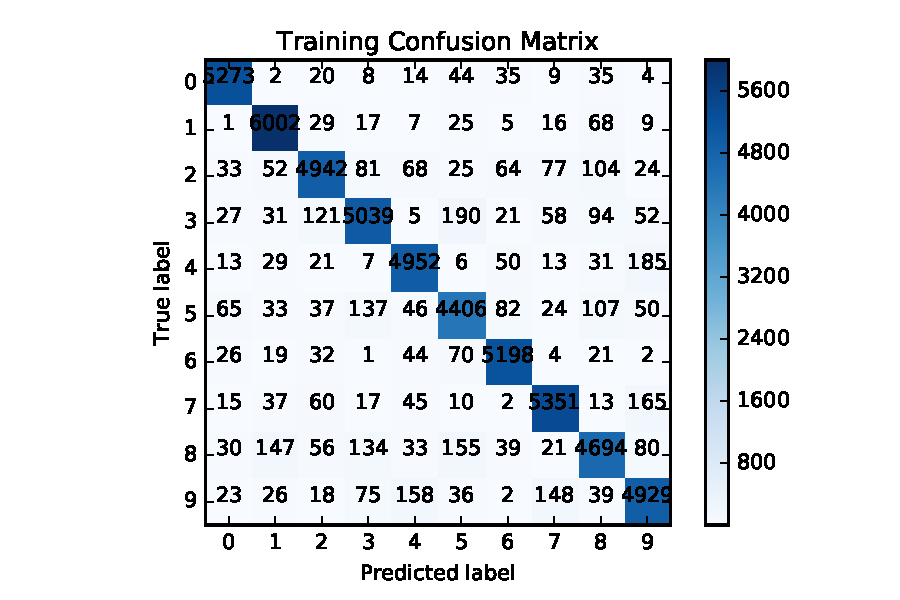
\includegraphics[width=0.85\textwidth]{./figures/train_pca.pdf}\
\caption{\label{fig:train_pca} Training Set Confusion Matrix Using PCA}
\end{figure}

\begin{figure}[H]
\centering
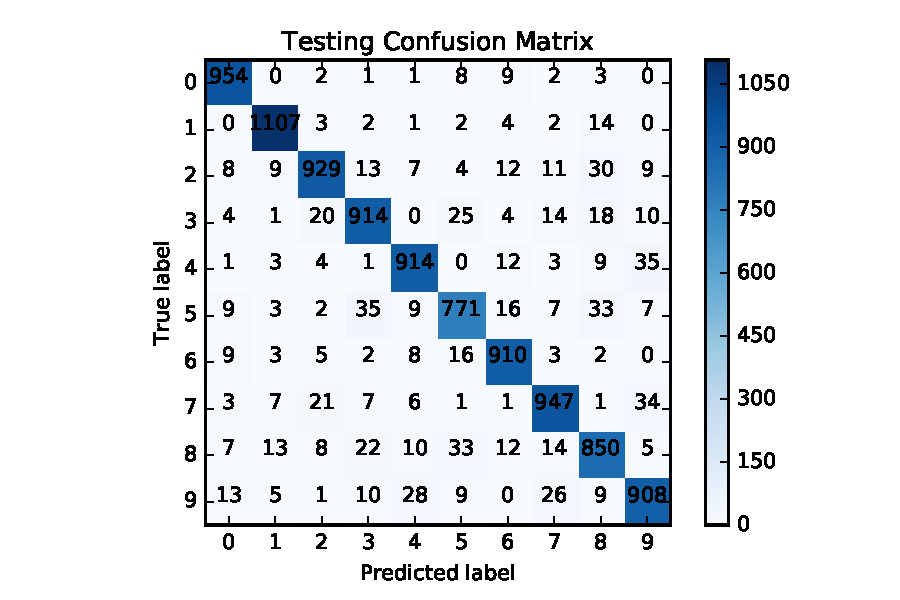
\includegraphics[width=0.85\textwidth]{./figures/test_pca.pdf}\
\caption{\label{fig:test_pca} Test Set Confusion Matrix Using PCA}
\end{figure}

(d). For the image processed by stacked RBM, the training and testing classification confusion matrix are shown in Figure \ref{fig:train_stack} and Figure \ref{fig:test_stack}.

\begin{figure}[H]
\centering
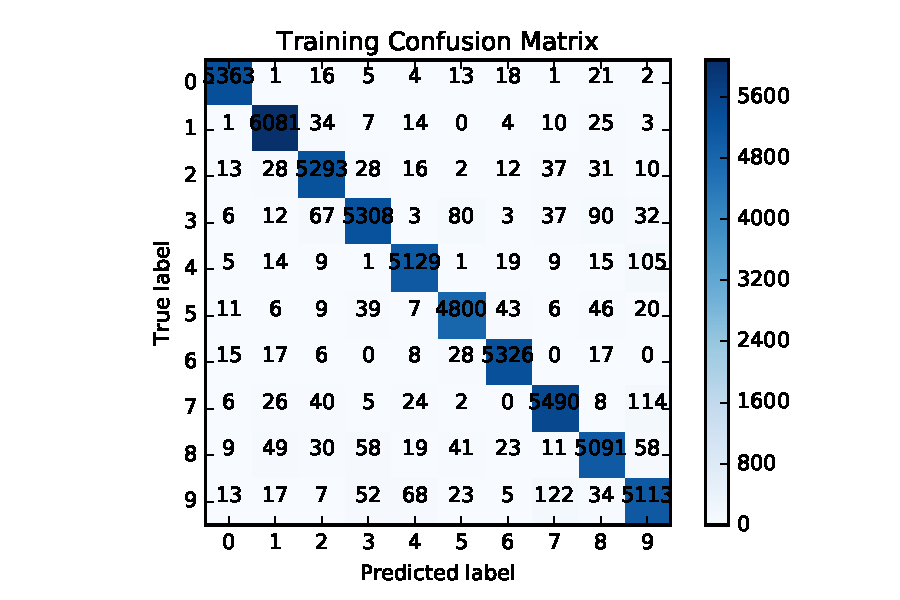
\includegraphics[width=0.85\textwidth]{./figures/train_stacking.pdf}\
\caption{\label{fig:train_stack} Training Set Confusion Matrix Using Stacked RBM}
\end{figure}

\begin{figure}[H]
\centering
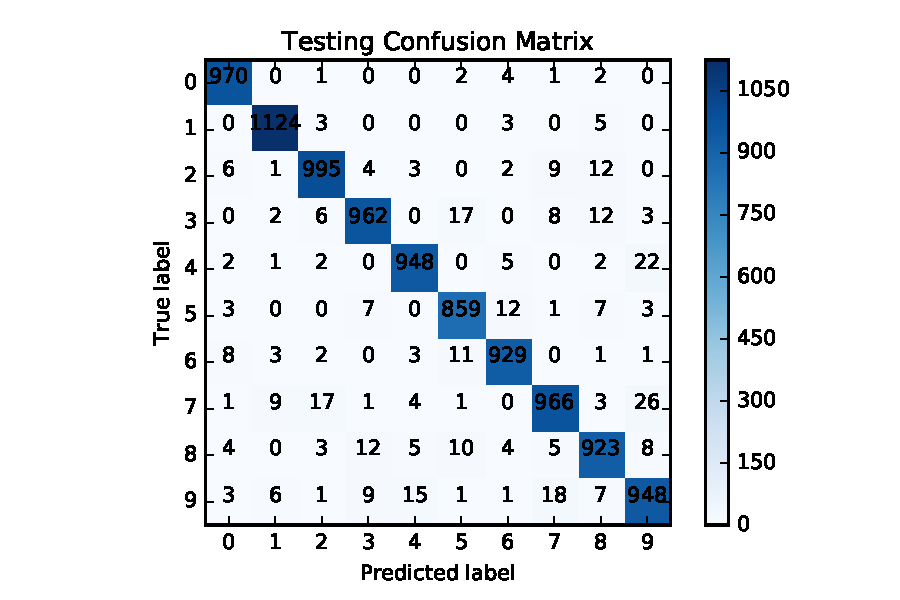
\includegraphics[width=0.85\textwidth]{./figures/test_stacking.pdf}\
\caption{\label{fig:test_stack} Test Set Confusion Matrix Using Stacked RBM}
\end{figure}


\clearpage
%\bibliographystyle{plain}
%\bibliographystyle{unsrt}
%\bibliography{reference.bib}

\end{document}

